\documentclass[9pt]{beamer}
\mode<presentation>

% Theme choice:
\usetheme{Madrid}%Darmstadt 

\usecolortheme[RGB={0,100,50}]{structure}
 \usefonttheme{structurebold} 
\setbeamercovered{invisible}
%\setbeamertemplate{navigation symbols}{}
\usepackage{dynblocks}
\usepackage{textpos}
\usepackage{amsfonts}
\usepackage{amsmath}
\usepackage{amssymb}
\usepackage{amsthm}

\newtheorem{teorema}{Teorema}\usepackage{mathtools}
\renewcommand{\proofname}{Prova}
\usepackage[portuguese]{babel}

\uselanguage{Portuguese}
\languagepath{Portuguese}

\deftranslation[to=Portuguese]{Theorem}{Teorema}
\deftranslation[to=Portuguese]{Lemma}{Lema}
\deftranslation[to=Portuguese]{Corollary}{Corolário}
\deftranslation[to=Portuguese]{Proof}{Prova}

\usepackage{dutchcal}
\usepackage{hyperref}
\usepackage[utf8]{inputenc}
\usepackage[T1]{fontenc}
\usepackage{amsthm}


\usepackage[affil-it]{authblk} 
\usepackage{etoolbox}
\usepackage{lmodern}

\makeatletter
\patchcmd{\@maketitle}{\LARGE \@title}{\fontsize{18}{19.2}\selectfont\@title}{}{}
\makeatother

\renewcommand\Authfont{\fontsize{12}{14.4}\selectfont}
\renewcommand\Affilfont{\fontsize{9}{10.8}\itshape}

% Title page details: 
\title[Presentation]{Lógica para Engenharia de Software} %add title


\institute[UniRV]{\textbf{\large  \textcolor{structure}{\textbf{\large
Teoria dos conjuntos: Definições iniciais, Conjunto Vazio, União e Interseção e provas matemáticas.
}} %add name 
% \hspace{0.5pt}
\\ \qquad
\\Professor: Me. Sergio Souza Novak 
\\Faculdade de Engenharia de Software}
} 
% \titlegraphic{\includegraphics[width=5cm]{msu.eps}}
\titlegraphic{
\includegraphics[width=5cm]{Universidade_de_Rio_Verde.jpg}}
\date{}

% Logo only on title page
%\logo{
\includegraphics[width=1cm,keepaspectratio]{Logo.png}}
\usepackage[pscoord]{eso-pic}


\begin{document}

% Title page frame
%\begin{frame}
    %\titlepage 
%\end{frame}
\frame[plain]{\titlepage}
%logo
\AddToShipoutPictureFG{
    \put(\LenToUnit{.92\paperwidth},
    \LenToUnit{.185\paperheight})
    {\vtop{{\null}
    \makebox{
\includegraphics[width=.8cm,keepaspectratio]{Universidade_de_Rio_Verde.jpg}}}}}


\begin{frame}{Sumário}
  \tableofcontents
\end{frame}


\section{Definição de conjuntos e representação }
\begin{frame}{Definição Formal de Conjuntos}

\begin{block}{Conjunto}
Um \textbf{conjunto} é uma coleção bem definida de elementos distintos, denominada por uma letra maiúscula, cujos elementos pertencem a um universo de discurso.
\end{block}

Seja $A$ um conjunto e $x$ um elemento qualquer. Dizemos que:
\[
x \in A \quad \text{se } x \text{ pertence a } A,
\]
\[
x \notin A \quad \text{se } x \text{ não pertence a } A.
\]

\begin{block}{Definição por Extensão}
Um conjunto pode ser definido listando explicitamente seus elementos:
\[
A = \{a_1, a_2, \dots, a_n\}.
\]
\end{block}

\begin{block}{Definição por Compreensão}
Um conjunto também pode ser definido por uma propriedade:
\[
A = \{\, x \in U \mid P(x) \,\},
\]
onde $U$ é o universo e $P(x)$ é uma proposição lógica.
\end{block}

\end{frame}
\begin{frame}{Conjuntos Definidos por Extensão}

\begin{block}{Definição por Extensão}
Um conjunto é definido por \textbf{extensão} quando seus elementos são explicitamente enumerados.
\end{block}

\begin{block}{Conjunto dos Números Pares (Extensão)}
O conjunto dos números pares pode ser definido como:
\[
P = \{0, 2, 4, 6, 8, \dots\}.
\]
\end{block}

\begin{block}{Observação}
A definição por extensão é adequada quando o conjunto é finito ou quando seus elementos seguem um padrão facilmente reconhecível.
\end{block}

\end{frame}
\begin{frame}{Conjuntos Definidos por Compreensão}

\begin{block}{Definição por Compreensão}
Um conjunto é definido por \textbf{compreensão} quando seus elementos são caracterizados por uma propriedade lógica.
\end{block}

\begin{block}{Conjunto dos Números Pares (Compreensão)}
O conjunto dos números pares pode ser definido como:
\[
P = \{\, x \in \mathbb{Z} \mid \exists k \in \mathbb{Z},\ x = 2k \,\}.
\]
\end{block}

\begin{block}{Observação}
A definição por compreensão permite descrever conjuntos infinitos de forma precisa e formal.
\end{block}

\end{frame}
\section{Conjunto Vazio}

\begin{frame}{Conjunto Vazio}
\begin{figure}[h]
    \centering
    
\includegraphics[width=0.1\linewidth]{conjunto_vazio.png}
    \caption{Conjunto vazio representado por um círculo sem elementos.}
    \label{fig:meu_grafico}
\end{figure}
\begin{block}{Definição}
O \textbf{conjunto vazio}, denotado por $\varnothing$ ou $\emptyset$, é o conjunto que não possui nenhum elemento.
\end{block}

\begin{block}{Caracterização Formal}
Um conjunto $A$ é vazio se, e somente se,
\[
\forall x,\; x \notin A.
\] 
\end{block} 

\begin{block}{Observação}
O conjunto vazio é único e é subconjunto de qualquer conjunto.
\end{block}

\end{frame}
\begin{frame}{Conjunto Vazio}

\begin{block}{Caracterização Formal}
Define-se o conjunto vazio, denotado por $\varnothing$, como o conjunto tal que
\[
\forall x,\; \bigl( x \in \varnothing \iff x \neq x \bigr).
\]
Equivalentemente,
\[
\varnothing = \{\, x \mid x \neq x \,\}.
\]
\end{block}

\begin{block}{Justificativa}
Como a proposição lógica $x \neq x$ é falsa para todo $x$, segue que
\[
\forall x,\; x \notin \varnothing.
\]
Logo, o conjunto $\varnothing$ não possui elementos.
\end{block}

\begin{block}{Observação}
O conjunto vazio é único e é subconjunto de qualquer conjunto, isto é,
\[
\forall A,\; \varnothing \subseteq A.
\]
\end{block}

\end{frame}


\begin{frame}{Exemplos de Conjunto Vazio}

\begin{block}{Exemplos}
Cada um dos conjuntos a seguir é vazio, pois nenhuma condição apresentada pode ser satisfeita:
\[
\begin{aligned}
A_1 &= \{\, x \in \mathbb{R} \mid x \neq x \,\} \\[4pt]
A_2 &= \{\, (x,y) \in \mathbb{R}^2 \mid 
\begin{cases}
x + y = 1 \\
x + y = 2
\end{cases} \,\} \\[6pt]
A_3 &= \{\, x \in \mathbb{N} \mid x < 0 \,\} \\[4pt]
A_4 &= \{\, x \in \mathbb{R} \mid x^2 < 0 \,\} \\[4pt]
\end{aligned}
\]
\end{block}

\end{frame} 
 
\begin{frame}{Exemplos de Conjunto Vazio}

\begin{block}{Exemplos}
Cada um dos conjuntos a seguir é vazio, pois nenhuma condição apresentada pode ser satisfeita:
\[
A_5 = \{\, x \in \mathbb{Z} \mid (\exists k \in \mathbb{Z},\ x = 2k)\ \land\ (\exists \ell \in \mathbb{Z},\ x = 2\ell + 1) \,\}
\]
\end{block}

\end{frame}
\begin{frame}{Cardinalidade de Conjuntos}

\begin{block}{Definição}
Seja $A$ um conjunto. Chama-se \textbf{cardinalidade} de $A$,
denotada por $|A|$, o número de elementos de $A$.
\end{block}

\begin{block}{Caracterização Formal}
Um conjunto $A$ é dito \textbf{finito} se existe um número natural $n \in \mathbb{N}$
tal que $A$ possui exatamente $n$ elementos.
Nesse caso, escreve-se
\[
|A| = n.
\]
\end{block}

\begin{block}{Observação}
Se não existe tal número natural, o conjunto é dito \textbf{infinito}.
\end{block}

\end{frame}
\begin{frame}{Exemplo de Conjunto Finito}

\begin{block}{Exemplo}
Considere o conjunto
\[
A = \{1, 3, 5, 7\}.
\]
\end{block}

\begin{block}{Análise}
O conjunto $A$ possui exatamente quatro elementos.
Logo, sua cardinalidade é
\[
|A| = 4.
\]
\end{block}

\begin{block}{Conclusão}
O conjunto $A$ é um conjunto finito.
\end{block}

\end{frame}
    \begin{frame}{Exemplo de Conjunto Infinito}

\begin{block}{Exemplo}
Considere o conjunto dos números naturais
\[
\mathbb{N} = \{0, 1, 2, 3, 4, \dots\}.
\]
\end{block}

\begin{block}{Análise}
Para qualquer número natural $n$, existe sempre um sucessor $n+1 \in \mathbb{N}$.
Assim, não é possível enumerar todos os seus elementos com um número finito.
\end{block}

\begin{block}{Conclusão}
O conjunto $\mathbb{N}$ é infinito.
\end{block}

\end{frame}
\begin{frame}{O Símbolo Seta}

\begin{block}{Motivação}
Em lógica e matemática, o símbolo seta é amplamente utilizado para expressar
\textbf{relações de dependência lógica} entre proposições.
\end{block}

\begin{block}{Ideia Intuitiva}
A expressão
\[
P \Rightarrow Q
\]
lê-se:
\begin{center}
\emph{``Se $P$ é verdadeiro, então $Q$ é verdadeiro.''}
\end{center}
\end{block}

\begin{block}{Uso em Matemática}
O símbolo $\Rightarrow$ aparece frequentemente em definições,
demonstrações e caracterizações formais.
\end{block}

\end{frame}
\begin{frame}{Definição Formal da Implicação}

\begin{block}{Definição}
Sejam $P$ e $Q$ proposições.
A implicação
\[
P \Rightarrow Q
\]
é verdadeira sempre que a veracidade de $P$ implica a veracidade de $Q$.
\end{block}

\begin{block}{Caracterização Lógica}
A implicação $P \Rightarrow Q$ é falsa \textbf{somente} no caso em que
$P$ é verdadeira e $Q$ é falsa.
\end{block}

\begin{block}{Observação}
Se $P$ é falsa, a implicação $P \Rightarrow Q$ é considerada verdadeira,
independentemente do valor lógico de $Q$.
\end{block}

\end{frame}
\begin{frame}{Exemplos de Implicação}

\begin{block}{Exemplo 1 — Aritmética}
Se $x$ é um número par, então $x^2$ é par:
\[
x \text{ é par } \Rightarrow x^2 \text{ é par}.
\]
\end{block}

\begin{block}{Exemplo 2 — Conjuntos}
Se um elemento pertence ao conjunto $A$ e $A \subseteq B$, então ele pertence a $B$:
\[
x \in A \Rightarrow x \in B.
\]
\end{block}

\begin{block}{Exemplo 3 — Definições}
A definição de subconjunto utiliza diretamente a implicação lógica:
\[
A \subseteq B \Rightarrow \forall x,\; (x \in A \Rightarrow x \in B).
\]
\end{block}

\end{frame}
\begin{frame}{Erros Comuns com o Símbolo Seta}

\begin{block}{Erro 1 — Confundir com Bicondicional}
A implicação
\[
P \Rightarrow Q
\]
não significa que $Q \Rightarrow P$ seja verdadeiro.
\end{block}

\begin{block}{Erro 2 — Confundir com Igualdade}
A expressão
\[
P \Rightarrow Q
\]
não significa que $P$ e $Q$ sejam equivalentes.
\end{block}

\begin{block}{Observação Final}
Quando ambos os sentidos são verdadeiros, utiliza-se o símbolo
\[
P \Leftrightarrow Q
\]
denominado \textbf{bicondicional}.
\end{block}

\end{frame}

\begin{frame}{Pertinência}
\begin{figure}[h]
    \centering
    
\includegraphics[width=0.6\linewidth]{pertence.png}
    \caption{Conjunto vazio representado por um círculo sem elementos.}
    \label{fig:meu_grafico}
\end{figure}
\begin{block}{Pertinência}
Seja $A$ um conjunto e $x$ um elemento.
Diz-se que $x$ \textbf{pertence} a $A$ se $x$ é um elemento de $A$,
o que se denota por
\[
x \in A.
\]
Caso contrário, escreve-se
\[
x \notin A.
\]
\end{block}

\end{frame}

\begin{frame}{Continência}

\begin{figure}[h]
    \centering
    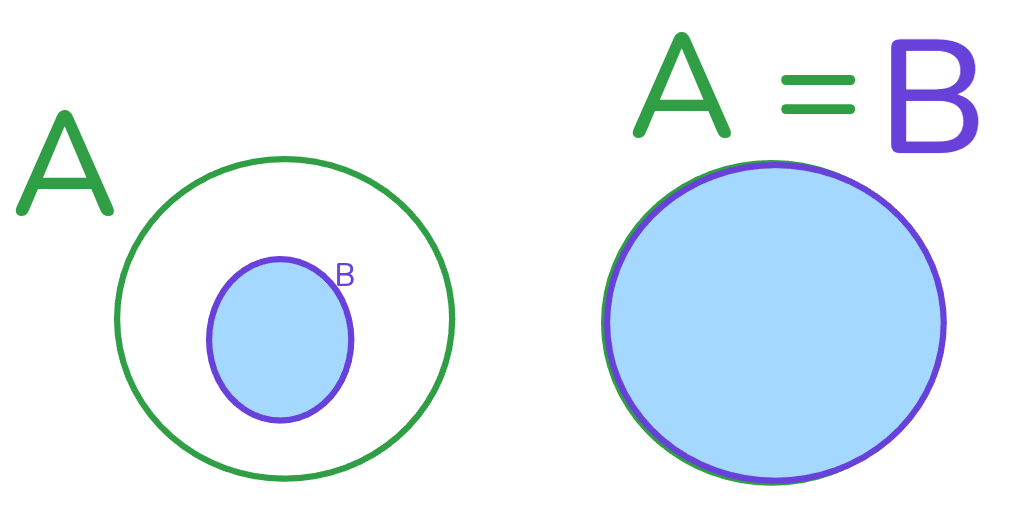
\includegraphics[width=0.6\linewidth]{contido.png}
    \caption{Conjunto A contém B representado por um círculo maior (A) contendo um círculo menor (B).}
    \label{fig:meu_grafico}
\end{figure}

\begin{block}{Continência}
Sejam $A$ e $B$ conjuntos.
Diz-se que $A$ está \textbf{contido} em $B$, ou que $A$ é subconjunto de $B$, se,
por definição,
\[
A \subseteq B \;\stackrel{\text{def}}{\Longleftrightarrow}\;
\forall x,\; (x \in A \Rightarrow x \in B).
\]
\end{block}
\end{frame}

\begin{frame}{Pertinência e Continência}

\begin{block}{Pertinência}
Seja $A$ um conjunto e $x$ um elemento.
Diz-se que $x$ \textbf{pertence} a $A$ se $x$ é um elemento de $A$,
o que se denota por
\[
x \in A.
\]
Caso contrário, escreve-se
\[
x \notin A.
\]
\end{block}

\begin{block}{Continência}
Sejam $A$ e $B$ conjuntos.
Diz-se que $A$ está \textbf{contido} em $B$, ou que $A$ é subconjunto de $B$, se,
por definição,
\[
A \subseteq B \;\stackrel{\text{def}}{\Longleftrightarrow}\;
\forall x,\; (x \in A \Rightarrow x \in B).
\]
\end{block}

\begin{block}{Observação Importante}
A pertinência relaciona \textbf{elemento–conjunto}, enquanto a continência relaciona
\textbf{conjunto–conjunto}.
Assim, $x \in A$ e $A \subseteq B$ são relações de naturezas distintas.
\end{block}

\end{frame}

\section{Igualdade de Conjuntos}

\begin{frame}{Igualdade de Conjuntos}

\begin{block}{Definição}
Sejam $A$ e $B$ conjuntos.  
Diz-se que $A$ e $B$ são \textbf{iguais} se possuem exatamente os mesmos elementos.
\end{block}

\begin{block}{Caracterização Formal}
\[
A = B 
\;\stackrel{\text{def}}{\Longleftrightarrow}\;
\forall x,\; (x \in A \Leftrightarrow x \in B).
\]
\end{block}

\begin{block}{Interpretação}
Dois conjuntos são iguais quando cada elemento de $A$ pertence a $B$  
e cada elemento de $B$ pertence a $A$.
\end{block}

\end{frame}
 

\begin{frame}{Igualdade e Dupla Inclusão}

\begin{block}{Teorema}
Para quaisquer conjuntos $A$ e $B$,
\[
A = B 
\;\Longleftrightarrow\;
(A \subseteq B \;\land\; B \subseteq A).
\]
\end{block}

\begin{block}{Demonstração (Ideia)}
\begin{itemize}
\item $(\Rightarrow)$ Se $A = B$, então todo elemento de $A$ está em $B$ e vice-versa.
\item $(\Leftarrow)$ Se $A \subseteq B$ e $B \subseteq A$, então possuem exatamente os mesmos elementos.
\end{itemize}
\end{block}

\begin{block}{Observação}
A igualdade de conjuntos é demonstrada, em geral, por meio da \textbf{dupla inclusão}.
\end{block}

\end{frame}
\begin{frame}{Exemplos de Igualdade de Conjuntos}

\begin{block}{Exemplo 1}
Considere:
\[
A = \{1,2,3\}
\quad
B = \{3,2,1\}.
\]
Como a ordem dos elementos não altera um conjunto,
\[
A = B.
\]
\end{block}

\begin{block}{Exemplo 2}
Considere:
\[
P = \{\, x \in \mathbb{Z} \mid x^2 = 1 \,\}
\quad
Q = \{-1,1\}.
\]
Logo,
\[
P = Q.
\]
\end{block}

\begin{block}{Observação}
A igualdade depende apenas dos elementos,  
não da ordem nem da forma de representação.
\end{block}

\end{frame}
\begin{frame}{Prova: $\varnothing \subseteq \varnothing$}

\begin{block}{Proposição}
O conjunto vazio está contido em si mesmo:
\[
\varnothing \subseteq \varnothing.
\]
\end{block}

\begin{block}{Prova}
Pela definição de subconjunto,
\[
A \subseteq B 
\;\stackrel{\text{def}}{\Longleftrightarrow}\;
\forall x,\; (x \in A \Rightarrow x \in B).
\]

Tomando $A = \varnothing$ e $B = \varnothing$, devemos verificar:
\[
\forall x,\; (x \in \varnothing \Rightarrow x \in \varnothing).
\]

Como não existe elemento $x$ tal que $x \in \varnothing$,  
a implicação é verdadeira para todo $x$.

Logo,
\[
\varnothing \subseteq \varnothing.
\]
\end{block}

\begin{block}{Observação} 
A proposição é verdadeira por \textbf{vacuidades lógica}:  
uma implicação com hipótese falsa é sempre verdadeira.
\end{block}

\end{frame}
\section{Interseção de conjuntos}

\begin{frame}{Definição de Interseção} 

\begin{block}{Definição}
Sejam $A$ e $B$ conjuntos.  
A \textbf{interseção} de $A$ e $B$ é o conjunto dos elementos
que pertencem simultaneamente a ambos.
\end{block}

\begin{block}{Notação}
\[
A \cap B
\]
\end{block}

\begin{block}{Caracterização Formal}
\[
x \in A \cap B
\;\stackrel{\text{def}}{\Longleftrightarrow}\;
(x \in A \land x \in B).
\]
\end{block}

\end{frame}
\begin{frame}{Interpretação Lógica da Interseção}

\begin{block}{Relação com a Lógica}
A interseção corresponde ao conectivo lógico
\textbf{conjunção} ($\land$).
\end{block}

\begin{block}{Leitura Formal}
\[
x \in A \cap B
\]
lê-se:
\begin{center}
"$x$ pertence a $A$ e pertence a $B$".
\end{center}
\end{block}

\begin{block}{Observação}
Se um elemento não pertence a um dos conjuntos,
então não pertence à interseção.
\end{block}

\end{frame}
\begin{frame}{Exemplos de Interseção}

\begin{block}{Exemplo 1}
Sejam
\[
A = \{1,2,3,4\}
\quad
B = \{3,4,5,6\}.
\]

Então,
\[
A \cap B = \{3,4\}.
\]
\end{block}

\begin{block}{Exemplo 2}
Sejam
\[
C = \{ x \in \mathbb{N} \mid x \text{ é par} \}
\]
\[
D = \{ x \in \mathbb{N} \mid x > 5 \}.
\]

Então,
\[
C \cap D = \{6,8,10,\dots\}.
\]
\end{block}

\end{frame}
\section{União}

\begin{frame}{Definição de União}

\begin{block}{Definição}
Sejam $A$ e $B$ conjuntos.  
A \textbf{união} de $A$ e $B$ é o conjunto dos elementos
que pertencem a pelo menos um dos conjuntos.
\end{block}

\begin{block}{Notação}
\[
A \cup B
\]
\end{block}

\begin{block}{Caracterização Formal}
\[
x \in A \cup B
\;\stackrel{\text{def}}{\Longleftrightarrow}\;
(x \in A \lor x \in B).
\]
\end{block}

\end{frame}
\begin{frame}{Interpretação Lógica da União}

\begin{block}{Relação com a Lógica}
A união corresponde ao conectivo lógico
\textbf{disjunção} ($\lor$).
\end{block}

\begin{block}{Leitura Formal}
\[
x \in A \cup B
\]
lê-se:
\begin{center}
"$x$ pertence a $A$ ou pertence a $B$".
\end{center}
\end{block}

\begin{block}{Observação}
Se o elemento pertence a ambos,
ele também pertence à união.
\end{block}

\end{frame}
\begin{frame}{Exemplos de União}

\begin{block}{Exemplo 1}
Sejam
\[
A = \{1,2,3\}
\quad
B = \{3,4,5\}.
\]

Então,
\[
A \cup B = \{1,2,3,4,5\}.
\]
\end{block}

\begin{block}{Exemplo 2}
Sejam
\[
E = \{ x \in \mathbb{Z} \mid x < 0 \}
\]
\[
F = \{ x \in \mathbb{Z} \mid x \geq 0 \}.
\]

Então,
\[
E \cup F = \mathbb{Z}.
\]
\end{block}

\end{frame}
\section{Provas envolvendo conjunto vazio}

\begin{frame}{Exercício 1 — Prova com Conjunto Vazio}

\begin{block}{Enunciado}
Prove que, para todo conjunto $A$,
\[
\varnothing \subseteq A.
\]
\end{block}

\begin{block}{Orientação}
Utilize a definição formal de subconjunto:
\[
A \subseteq B 
\Longleftrightarrow 
\forall x,\; (x \in A \Rightarrow x \in B).
\]
\end{block}

\begin{block}{Dica}
Analise o valor lógico da implicação quando
$x \in \varnothing$.
\end{block}

\end{frame}
\begin{frame}{Exercício 2 — Interseção com $\varnothing$}

\begin{block}{Enunciado}
Prove que, para todo conjunto $A$,
\[
A \cap \varnothing = \varnothing.
\]
\end{block}

\begin{block}{Orientação}
Mostre dupla inclusão:
\[
A \cap \varnothing \subseteq \varnothing
\quad \text{e} \quad
\varnothing \subseteq A \cap \varnothing.
\]
\end{block}

\begin{block}{Dica}
Use a definição:
\[
x \in A \cap B \Longleftrightarrow (x \in A \land x \in B).
\]
\end{block}

\end{frame}
\begin{frame}{Exercício 3 — União com $\varnothing$}

\begin{block}{Enunciado}
Prove que, para todo conjunto $A$,
\[
A \cup \varnothing = A.
\]
\end{block}

\begin{block}{Orientação}
Demonstre por dupla inclusão.
\end{block}

\begin{block}{Dica}
Utilize:
\[
x \in A \cup B 
\Longleftrightarrow 
(x \in A \lor x \in B).
\]
\end{block}

\end{frame}
\begin{frame}{Exercício 4 — Subconjuntos do Vazio}

\begin{block}{Enunciado}
Prove que, se $A \subseteq \varnothing$, então
\[
A = \varnothing.
\]
\end{block}

\begin{block}{Orientação}
Suponha que exista $x \in A$ e derive contradição.
\end{block}

\begin{block}{Dica}
Lembre-se de que
\[
\forall x,\; x \notin \varnothing.
\]
\end{block}

\end{frame}\begin{frame}{Exercício 5 — Interseção Vazia}

\begin{block}{Enunciado}
Se $A \cap B = \varnothing$, prove que
\[
\forall x,\; (x \in A \Rightarrow x \notin B).
\]
\end{block}

\begin{block}{Orientação}
Use a definição de interseção e raciocínio por contradição.
\end{block}

\begin{block}{Objetivo Conceitual}
Interpretar interseção vazia como
\textbf{ausência de elementos em comum}.
\end{block}

\end{frame}
\begin{frame}{Respostas — Provas com $\varnothing$ (Parte 1 — Versão Formal)}

\begin{block}{(1) $\varnothing \subseteq A$}
Por definição,
\[
\varnothing \subseteq A 
\Longleftrightarrow 
\forall x\, (x \in \varnothing \Rightarrow x \in A).
\]

Fixe $x$ arbitrário.
A proposição $x \in \varnothing$ é falsa.
Logo, a implicação
\[
x \in \varnothing \Rightarrow x \in A
\]
é verdadeira.

Como $x$ foi arbitrário, segue
\[
\forall x\, (x \in \varnothing \Rightarrow x \in A).
\]

Portanto, $\varnothing \subseteq A$.
\end{block}

\begin{block}{(2) $A \cap \varnothing = \varnothing$}
Provaremos dupla inclusão.

\textbf{(i)} $A \cap \varnothing \subseteq \varnothing$

Seja $x \in A \cap \varnothing$.
Então,
\[
x \in A \land x \in \varnothing.
\]
Mas não existe $x$ tal que $x \in \varnothing$.
Logo, tal $x$ não existe.
Portanto,
\[
A \cap \varnothing \subseteq \varnothing.
\]
\end{block}

\end{frame}\begin{frame}{Respostas — Provas com $\varnothing$ (Continuação)}

\begin{block}{(2) Continuação}
\textbf{(ii)} $\varnothing \subseteq A \cap \varnothing$

Pelo item (1), o conjunto vazio é subconjunto de qualquer conjunto.
Logo,
\[
\varnothing \subseteq A \cap \varnothing.
\]

Concluímos, pela dupla inclusão,
\[
A \cap \varnothing = \varnothing.
\]
\end{block}

\begin{block}{(3) $A \cup \varnothing = A$}
Provaremos dupla inclusão.

\textbf{(i)} $A \cup \varnothing \subseteq A$

Seja $x \in A \cup \varnothing$.
Então,
\[
x \in A \lor x \in \varnothing.
\]
Como $x \in \varnothing$ é impossível, segue $x \in A$.
Logo,
\[
A \cup \varnothing \subseteq A.
\]
\end{block}

\end{frame}
% \begin{frame}{Prova: $\varnothing \subseteq A$}

% \begin{block}{Proposição}
% Para todo conjunto $A$, vale:
% \[
% \varnothing \subseteq A.
% \]
% \end{block}

% \begin{block}{Prova}
% Pela definição de subconjunto,
% \[
% \varnothing \subseteq A 
% \Longleftrightarrow 
% \forall x,\; (x \in \varnothing \Rightarrow x \in A).
% \]

% Como não existe elemento $x$ tal que $x \in \varnothing$,  
% a implicação é sempre verdadeira.

% Logo,
% \[
% \varnothing \subseteq A.
% \]
% \end{block}

% \begin{block}{Observação}
% Trata-se novamente de uma verdade por vacuidade lógica.
% \end{block}

% \end{frame}
\end{document}
